\documentclass{beamer}

% Preamble
\usetheme{Copenhagen}
\usecolortheme{seagull}
\usefonttheme[onlysmall]{structurebold}
\setbeamerfont{title}{shape=\itshape,family=\rmfamily}
\setbeamertemplate{footline}[frame number]
\usepackage[absolute,overlay]{textpos}
\useinnertheme{circles}
\usepackage{tikz,overpic}
\usepackage{courier}
\usepackage{verbatim}
\usetikzlibrary{fit,shapes.misc,arrows, shapes}
\usepackage{varwidth}
\usepackage[latin1]{inputenc}
\usepackage[T1]{fontenc}
\usepackage{libertine}
\usepackage{graphicx}
\PassOptionsToPackage{svgnames}{xcolor}
\usepackage{framed}
\usepackage{animate}

% put the text at the right corner
\newcommand\FrameText[1]{%
\begin{textblock*}{\paperwidth}(0pt,\textheight)
	\raggedright #1\hspace{.5em}
\end{textblock*}}

% divide slide into 4
\newcommand\FourQuad[4]{%
    \begin{minipage}[b][.35\textheight][t]{.47\textwidth}#1\end{minipage}\hfill%
    \begin{minipage}[b][.35\textheight][t]{.47\textwidth}#2\end{minipage}\\[0.5em]
    \begin{minipage}[b][.35\textheight][t]{.47\textwidth}#3\end{minipage}\hfill
    \begin{minipage}[b][.35\textheight][t]{.47\textwidth}#4\end{minipage}%
}


%quote
\newcommand*\openquote{\makebox(7,3){\scalebox{5.}{``}}}
%for the close quote
%\newcommand*\closequote{\makebox(25,-22){\scalebox{5}{''}}}
\colorlet{shadecolor}{white}
\makeatletter
\newif\if@right
\def\shadequote{\@righttrue\shadequote@i}
\def\shadequote@i{\begin{snugshade}\begin{quote}\openquote}
\def\endshadequote{%
	\if@right\hfill\fi\end{quote}\end{snugshade}}
    %\if@right\hfill\fi\closequote\end{quote}\end{snugshade}}
\@namedef{shadequote*}{\@rightfalse\shadequote@i}
\@namedef{endshadequote*}{\endshadequote}
\makeatother


%change fontsize
\newcommand\Fontvi{\fontsize{6}{7.2}\selectfont}

% title page
\title{?`Do We Have Black Chromatin?}
       

\author[Lim]
{Ricky Lim\inst{1, 2} }
\institute[] 
{
	\inst{1}
	FNWI\\
	Universiteit van Amsterdam
	\and
 	\inst{2}
  	Genome Architecture \& Bioinformatics\\
  	Centre for Genomic Regulation (CRG)
}
\date[10 June 2012]
{Master Thesis Presentation\\\tiny{mailto:rickylim19@gmail.com}}


\subject{Master Thesis Presentation}

% start presenting...
\begin{document}

\begin{frame}
\titlepage
\end{frame}

\begin{frame}
\frametitle{Acknowledgments}
	\begin{shadequote}
        		\Fontvi A dream you dream alone is only a dream. A dream you dream together is reality. -Yoko Ono
	\end{shadequote}
	
	 \begin{itemize}
          	\item \textbf{Supervisors:}
          		  \begin{itemize}
	 				\item Dr. Guillaume Filion
					\item Dr. Hans van der Spek
				  \end{itemize}
			\item \textbf{Team Players:}
			      \begin{itemize}
	 				\item Heng-Chang Chen, Dr. rer. nat. (Ph.D.)
					\item Marc Corrales
					\item Dr. Olivera Vujatovi
					\item Catarina De Oliveira					  
				 \end{itemize}
			\item \textbf{Fellowships:}
				 \begin{itemize}
	 				\item Fontane
					\item Huygens Scholarship Programme
					\item Erasmus Programme
				  \end{itemize}
	\end{itemize}
\end{frame}

\begin{frame}
	\frametitle{Today's Menu}
	\tableofcontents
\end{frame}


\begin{frame}
	\pause
	\tikzstyle{block} = [rectangle, draw, fill=gray!20, 
    text width=\textwidth, text centered, rounded corners, minimum height=4em]
	\begin{tikzpicture}[node distance = 2cm, auto]
    \node [block] () {Prelude};
	\end{tikzpicture}
\end{frame}

\section{Prelude}
\begin{frame}
	\frametitle{Top 10  Most Frequent Words}
	\pause
	\begin{figure}
   			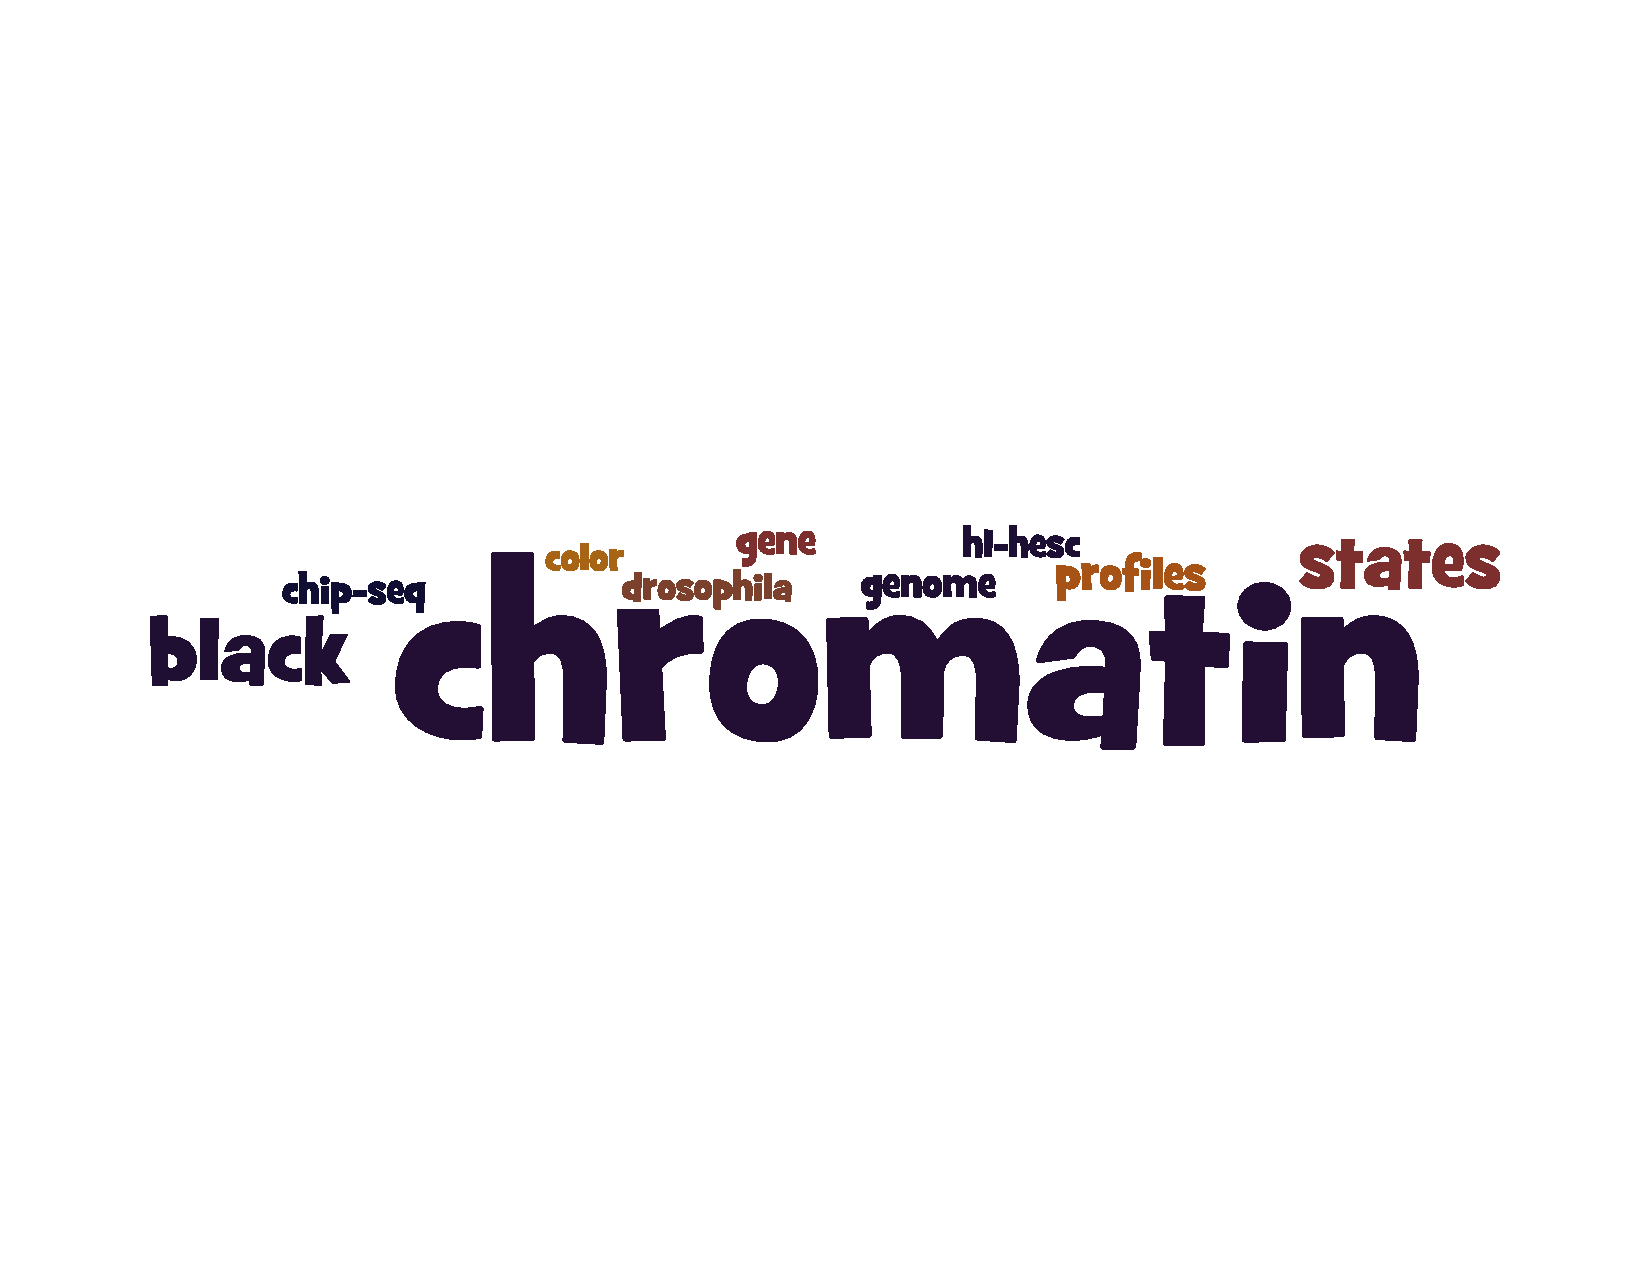
\includegraphics[width=1\textwidth]{figs/Top10.pdf}
 	\end{figure}
\end{frame}

\begin{frame}
	\frametitle{Summary in 4 Sentences}
	\pause
	\begin{itemize}[<+->]
		\item In 2010, a work by Filion and colleagues proposed that the genome is segmented genome-wide into five major chromatin types in Drosophila. 
		\item Among these five states, they identified a novel repressive chromatin covering about half of the genome and without the presence of the known heterochromatin markers HP1 and Polycomb. 
		\item Here, we present a genome-wide chromatin landscape in Human H1-hESC based on 68 chromatin features covering histone modifications and transcription factors. 
		\item Further supported by other datasets (Lamina-associated domains, CpG islands, RefSeq gene and exon, open chromatin, and RNA-seq), we confirm the existence of Black chromatin among these four major chromatin types in Human.
	\end{itemize}
\end{frame}

\section{Introduction}
\begin{frame}
	\pause
	\tikzstyle{block} = [rectangle, draw, fill=gray!20, 
    text width=\textwidth, text centered, rounded corners, minimum height=4em]
	\begin{tikzpicture}[node distance = 2cm, auto]
    \node [block] () {Introduction};
	\end{tikzpicture}
\end{frame}

% what is black?
\begin{frame}
	\frametitle{Black Chromatin: Revisited}
 	\begin{columns}
 		\begin{column}{.48\textwidth}
			\begin{shadequote}
        		\Fontvi Chromatin state is a segmentation of the genome based on a unique combination of chromatin proteins. 
       	\end{shadequote}
  		\begin{figure}
   			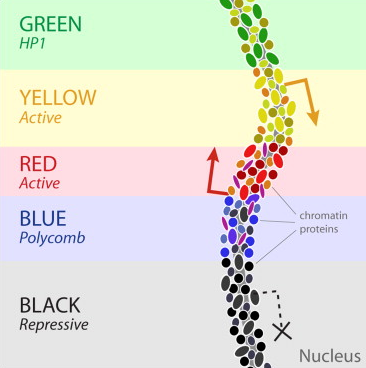
\includegraphics[width=.7\textwidth]{figs/ColorChromatin}
  		\end{figure}

  		\pause
 		\end{column}
 		\begin{column}{.48\textwidth} 
  			\alert{Black Chromatin}: a novel type of repressive chromatin
			\pause
			 \begin{itemize}[<+->]
   	 			\item Hardly no binding of chromatin proteins
          		\item Black covers 48\% of the genome
          		\item Harboring $\approx$ 4000 genes that are linked to developmental regulation
  			\end{itemize}
 		\end{column}
 	\end{columns}
 	
	\footnote{(Filion et al., 2010)}
  	\note{Color-coded classification, five principle types}
  	\note{genomic regions: 1kb to 100kb}
	\note{4,000 genes lack of any known inactive chromatin marks and transcriptional repressors}
\end{frame}

\subsection{?`Our Question?}
\begin{frame}
	\frametitle{Yes$\mid$No}
	\pause
	\tikzstyle{block} = [rectangle, draw, fill=gray!20, 
    text width=\textwidth, text centered, rounded corners, minimum height=4em]

	\begin{tikzpicture}[node distance = 2cm, auto]
    \node [block] (question) {So far Black was only identified in {\it Drosophila}...\\ \textbf{Does Black also present in Humans?}};
	\end{tikzpicture}
\end{frame}

\subsection{Our Strategy}
\begin{frame}
	\frametitle{Our Strategy}
	\begin{columns}
 		\begin{column}{.48\textwidth}
			\begin{figure}
				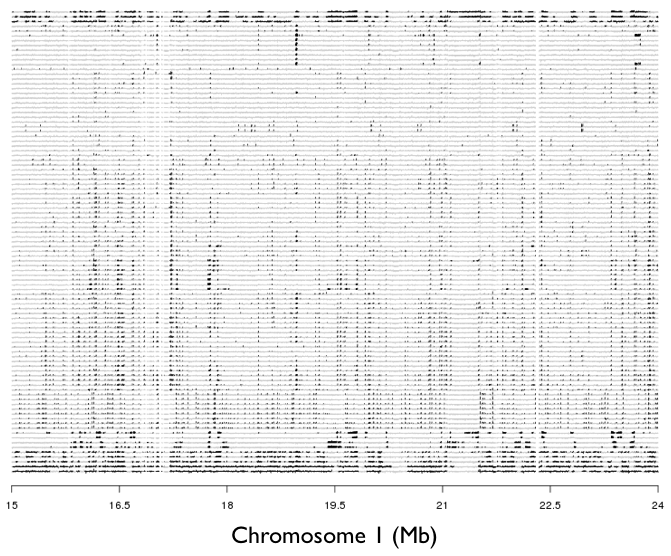
\includegraphics[width=1.\textwidth]{figs/mat}
			\end{figure}
		\end{column}
		\pause
 		\begin{column}{.48\textwidth}
			\begin{figure}
				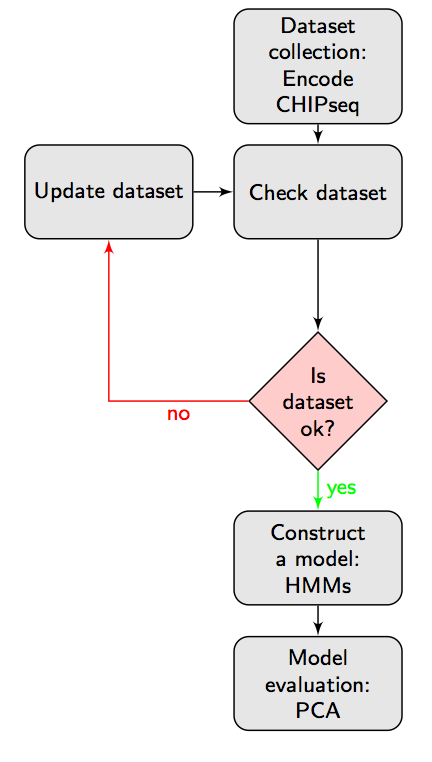
\includegraphics[width=.7\textwidth]{figs/strategy}
			\end{figure}
		\end{column}
	
	\end{columns}
\end{frame}

\section{Our Results}
\begin{frame}
	\frametitle{4 Chromatin States in H1-hESC 
	   \href{http://lab.thegrandlocus.com/static/images/human_4color.gif}{\beamergotobutton{Animated here}}}

			\begin{figure}
				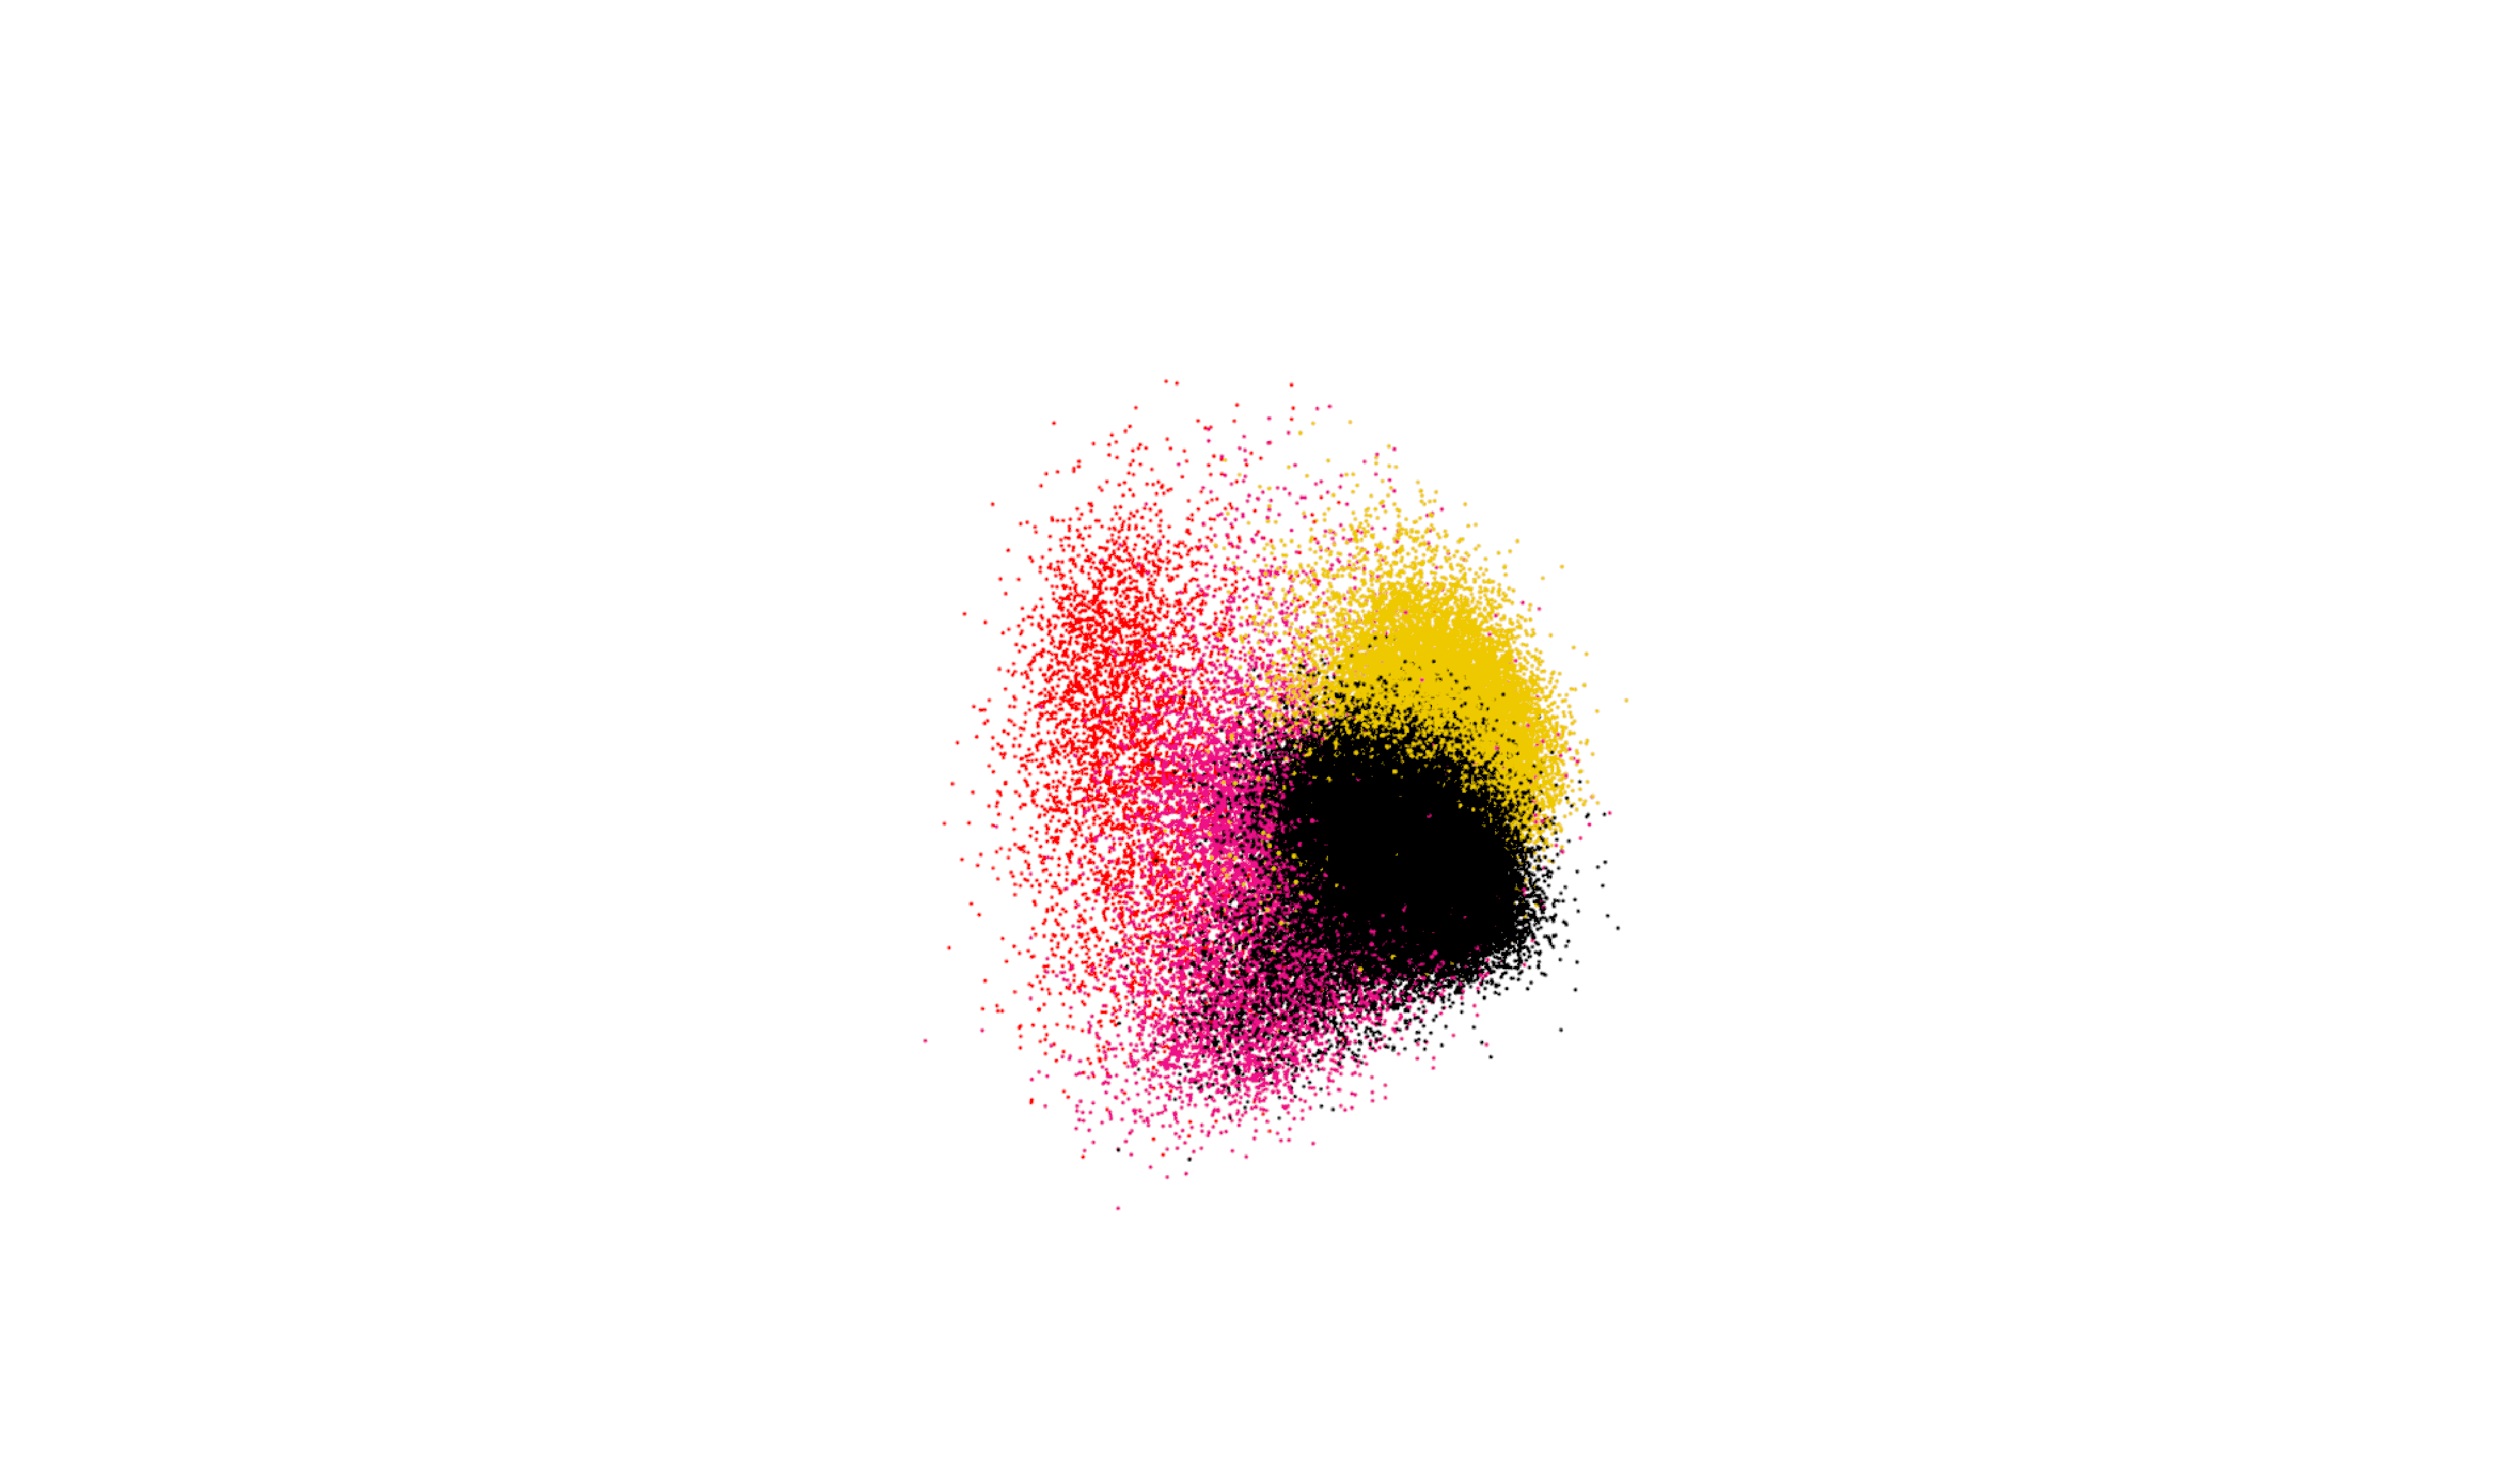
\includegraphics[width=1.0\textwidth]{figs/PCA4Color}
			\end{figure}
			

\end{frame}

\begin{frame}
	\frametitle{Black Is among Our Four Chromatin States}
	\begin{figure}
   			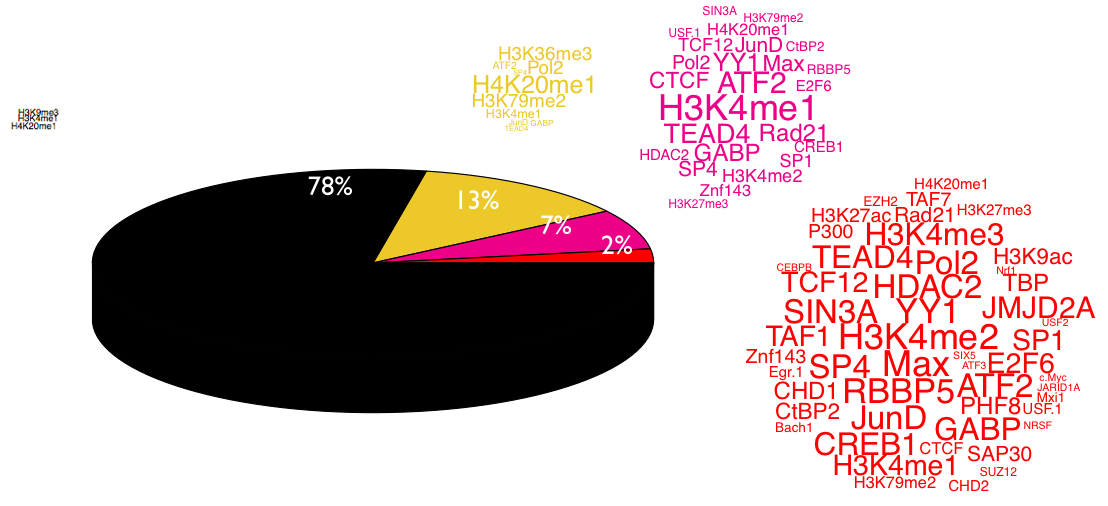
\includegraphics[width=1\textwidth]{figs/3Dpizza}
    \end{figure}

\end{frame}

\begin{frame}
\begin{columns}
\frametitle{Features of Black Chromatin}
		\pause
 		\begin{column}{.5\textwidth}
		\begin{figure}
   			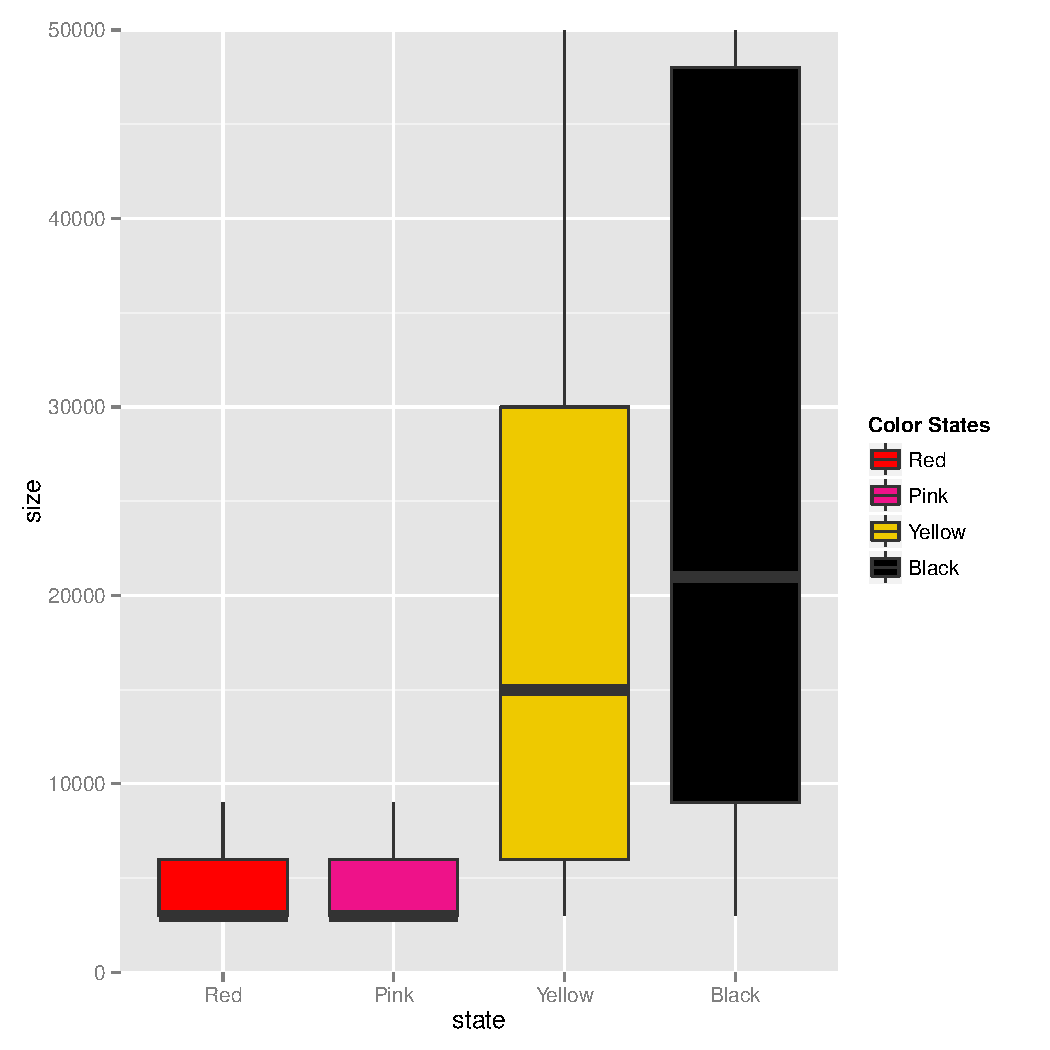
\includegraphics[width=1.\textwidth]{figs/domain_size}
  		\end{figure}
		\end{column}
		
		\pause
		\begin{column}{.5\textwidth}
		\begin{figure}
   			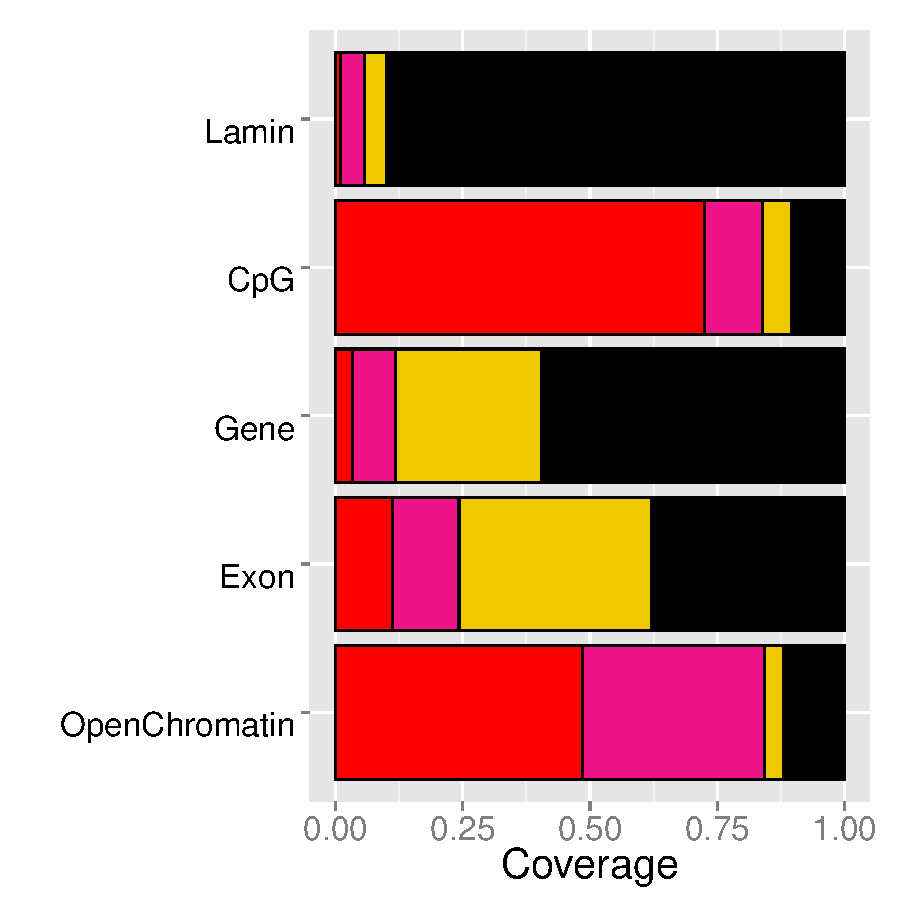
\includegraphics[width=1.\textwidth]{figs/AllFeatureCoverage}
  		\end{figure}
		
		\end{column}
	\end{columns}
\end{frame}

\begin{frame}
\begin{columns}
\frametitle{Expression Levels of Black Chromatin}
		\pause
 		\begin{column}{.5\textwidth}
		\begin{figure}
   			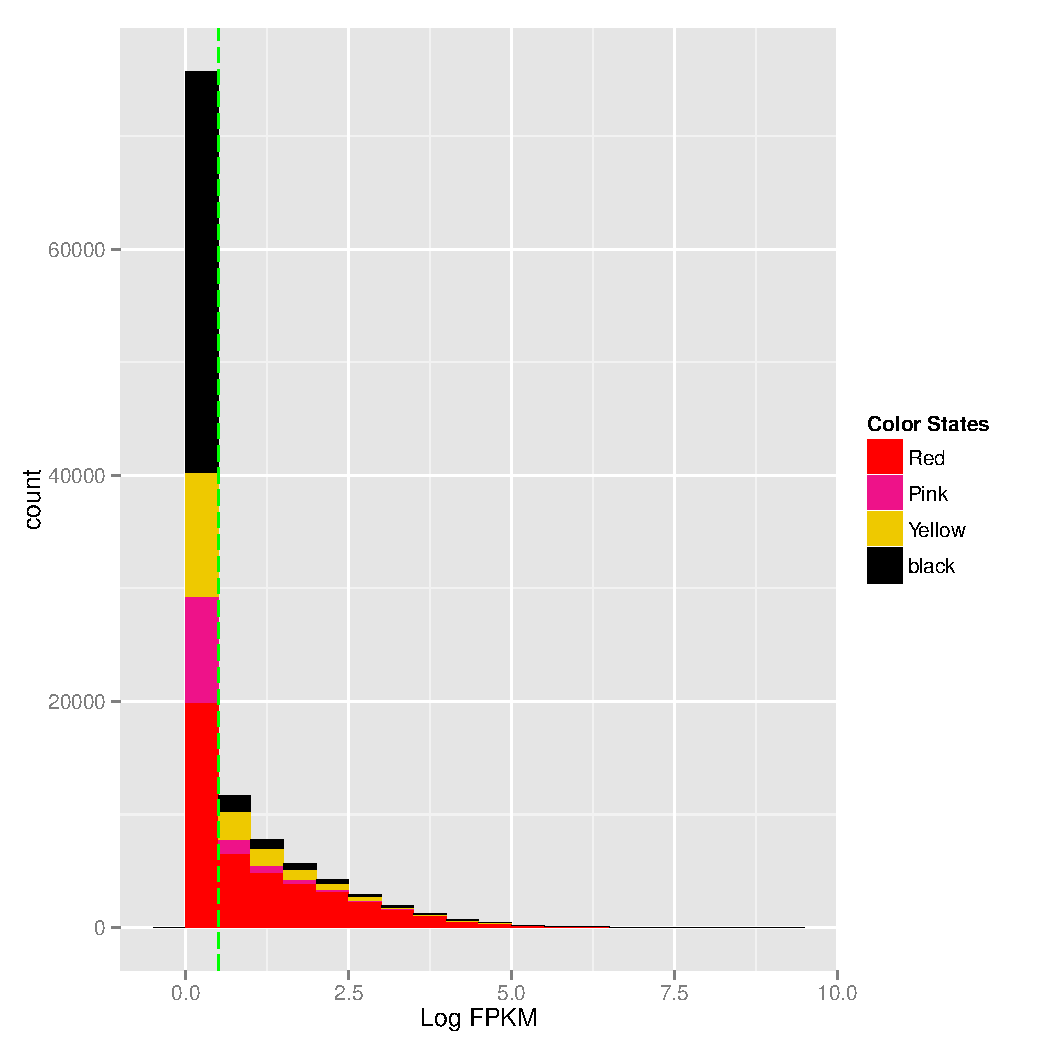
\includegraphics[width=1.\textwidth]{figs/TSSFPKM}
  		\end{figure}
		\end{column}
	
		\begin{column}{.5\textwidth}
		\begin{figure}
   			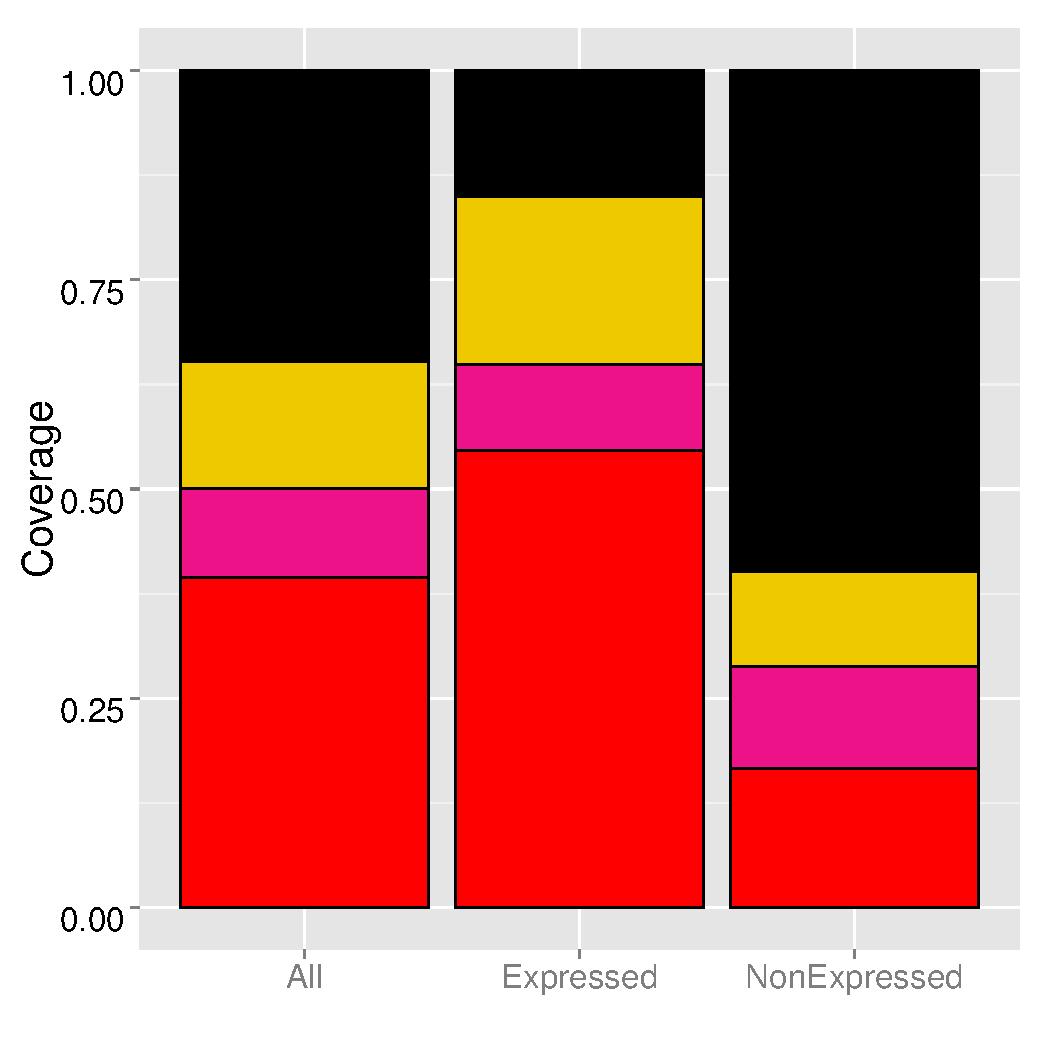
\includegraphics[width=1.\textwidth]{figs/TSSnpIDR}
  		\end{figure}
		
		\end{column}
	\end{columns}
\end{frame}

\begin{frame}
	\frametitle{Black Points toward Facultative Biological Process}
	\pause
	\begin{figure}
   			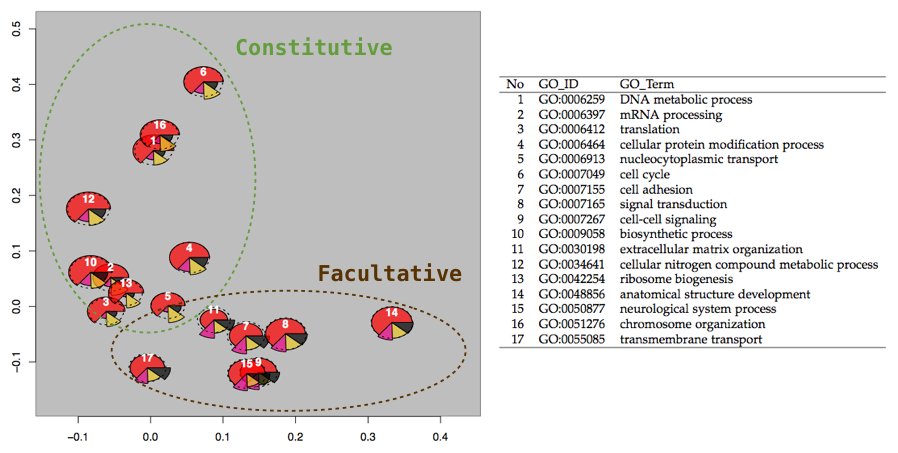
\includegraphics[width=1\textwidth]{figs/GOSpie}
    \end{figure}

\end{frame}

\section{Conclusion}
\begin{frame}
	\frametitle{Conclusion}
	\begin{itemize}[<+->]
   	 	  \item Utility of integrative analysis in Chromatin of H1-hESC
		  \item ?`Do We have Black Chromatin?
		  \begin{itemize}
          	\item \textbf{Yes}, we have
		  \end{itemize}
          \item \textbf{Future perspectives:}
          \begin{itemize}[<+->]
          	\item Mechanistic explanations of Black Chromatin in Human?
          	\item Going forward from a normal $\rightarrow$ disease condition?
		  \end{itemize}
  	\end{itemize}
\end{frame}

\begin{frame}
	\begin{figure}
		
\includegraphics[width=0.7\textwidth]{figs/BlackBatman}
	\end{figure}
\end{frame}

\begin{frame}
	\frametitle{Q\&A}
	\begin{figure}
		
\includegraphics[width=1\textwidth]{figs/Q&A}
	\end{figure}
\end{frame}

\end{document}